\documentclass[%
 aip,
% jmp,
% bmf,
% sd,
% rsi,
cp,  % Conference Proceedings
 amsmath,amssymb,%nobibnotes,
% preprint,%
 reprint,%
%author-year,%
%author-numerical,%
]{revtex4-2}

\usepackage{graphicx}% Include figure files
\usepackage{dcolumn}% Align table columns on decimal point
\usepackage{bm}% bold math
%\usepackage[mathlines]{lineno}% Enable numbering of text and display math
%\linenumbers\relax % Commence numbering lines

\usepackage[utf8]{inputenc}
\usepackage[T1]{fontenc}
%% Loads a Times-like font. You can also load
%% {newtxtext,newtxtmath}, but not {times}, 
%% {txfonts} nor {mathtpm} as these packages
%% are obsolete and have been known to cause problems.
\usepackage{mathptmx} 

% My package
\usepackage{overpic}
\usepackage{hyperref}

\begin{document}

\title{Reactor like TGE model}% Force line breaks with \\

\author{Mikhail Zelenyi} % Write as First name Surname
\email[Corresponding author: ]{mihail.zelenyy@phystech.edu}
\affiliation{
Moscow Institute of Physics and Technology}
\affiliation{%
Institute for Nuclear Research of RAS
}%
\affiliation{
Space Research Institute of RAS
}
\author{Alexander Nozik}%
\email{altavir@gmail.com}
\author{Egor Stadnichuk}
\email{egrstadnichuk@yandex.ru}
\affiliation{
Moscow Institute of Physics and Technology}
\affiliation{%
Institute for Nuclear Research of RAS
}%


\date{\today} % It is always \today, today, but any date may be explicitly specified
              % Not printed for conference proceedings

\begin{abstract}
Terrestrial gamma flash (TGF) and thunderstorm ground enhancements(TGE) phenomena are crucial for understanding of atmosphere breakdown and lightning generation physics. The initial theory was developed by Gurevich and included only runway breakdown description. It was later updated by Babich and Dwayer, but even updated models use a rather simplified field structure and do not fully explain observed quantities. The reactor like TGE (RL-TGE) model presented in this work assumes more complicated stochastic field structure and takes into account not only one cell runway breakdown, but the whole global field cellular structure in the thundercloud. It allows to describe a wide variety of TGF-like events and potentially fills the gap in thundercloud parameters previously unaccounted by other theories.
\end{abstract}

\maketitle

\section{Introduction}
Many previous works point to the fact that electric field inside the thundercloud is high enough to accelerate electrons and produce secondary electromagnetic showers ~\cite{gurevich1992runaway, gurevich1999lightning,dwyer2003fundamental,dwyer2011low,gurevich2001kinetic, dwyer2015positron, dwyer2013properties}.
The acceleration of electron is possible under two conditions:
\begin{itemize}
    \item The strength of the field is higher than so-called critical field. The value of the critical field equals energy loss of minimally ionizing electron per length unit.
    \item The initial electron energy is high enough to be close to minimally ionizing energy.
\end{itemize}
The major problem of all of these models is that while field strength is higher than critical field, the multiplication coefficient for showers is rather small and can’t describe some observed effects~\cite{npm_dwyer, Stadnichuk}. To solve these problems in this article we would like to present a concept of model describing a set of phenomena occurring in thundercloud, which is based on a combined global simulation of electron and photon transport inside the whole volume of the thundercloud.
\section{Reactor like TGE model}
\begin{figure}
    \centering
    \begin{overpic}[scale=.5]{figures/electric_streams.pdf}
    \put(15,53){\includegraphics[scale=.015]{figures/cell.pdf}}
    \put(20,69){\text{Acceleration cell}}
    \put(10,10){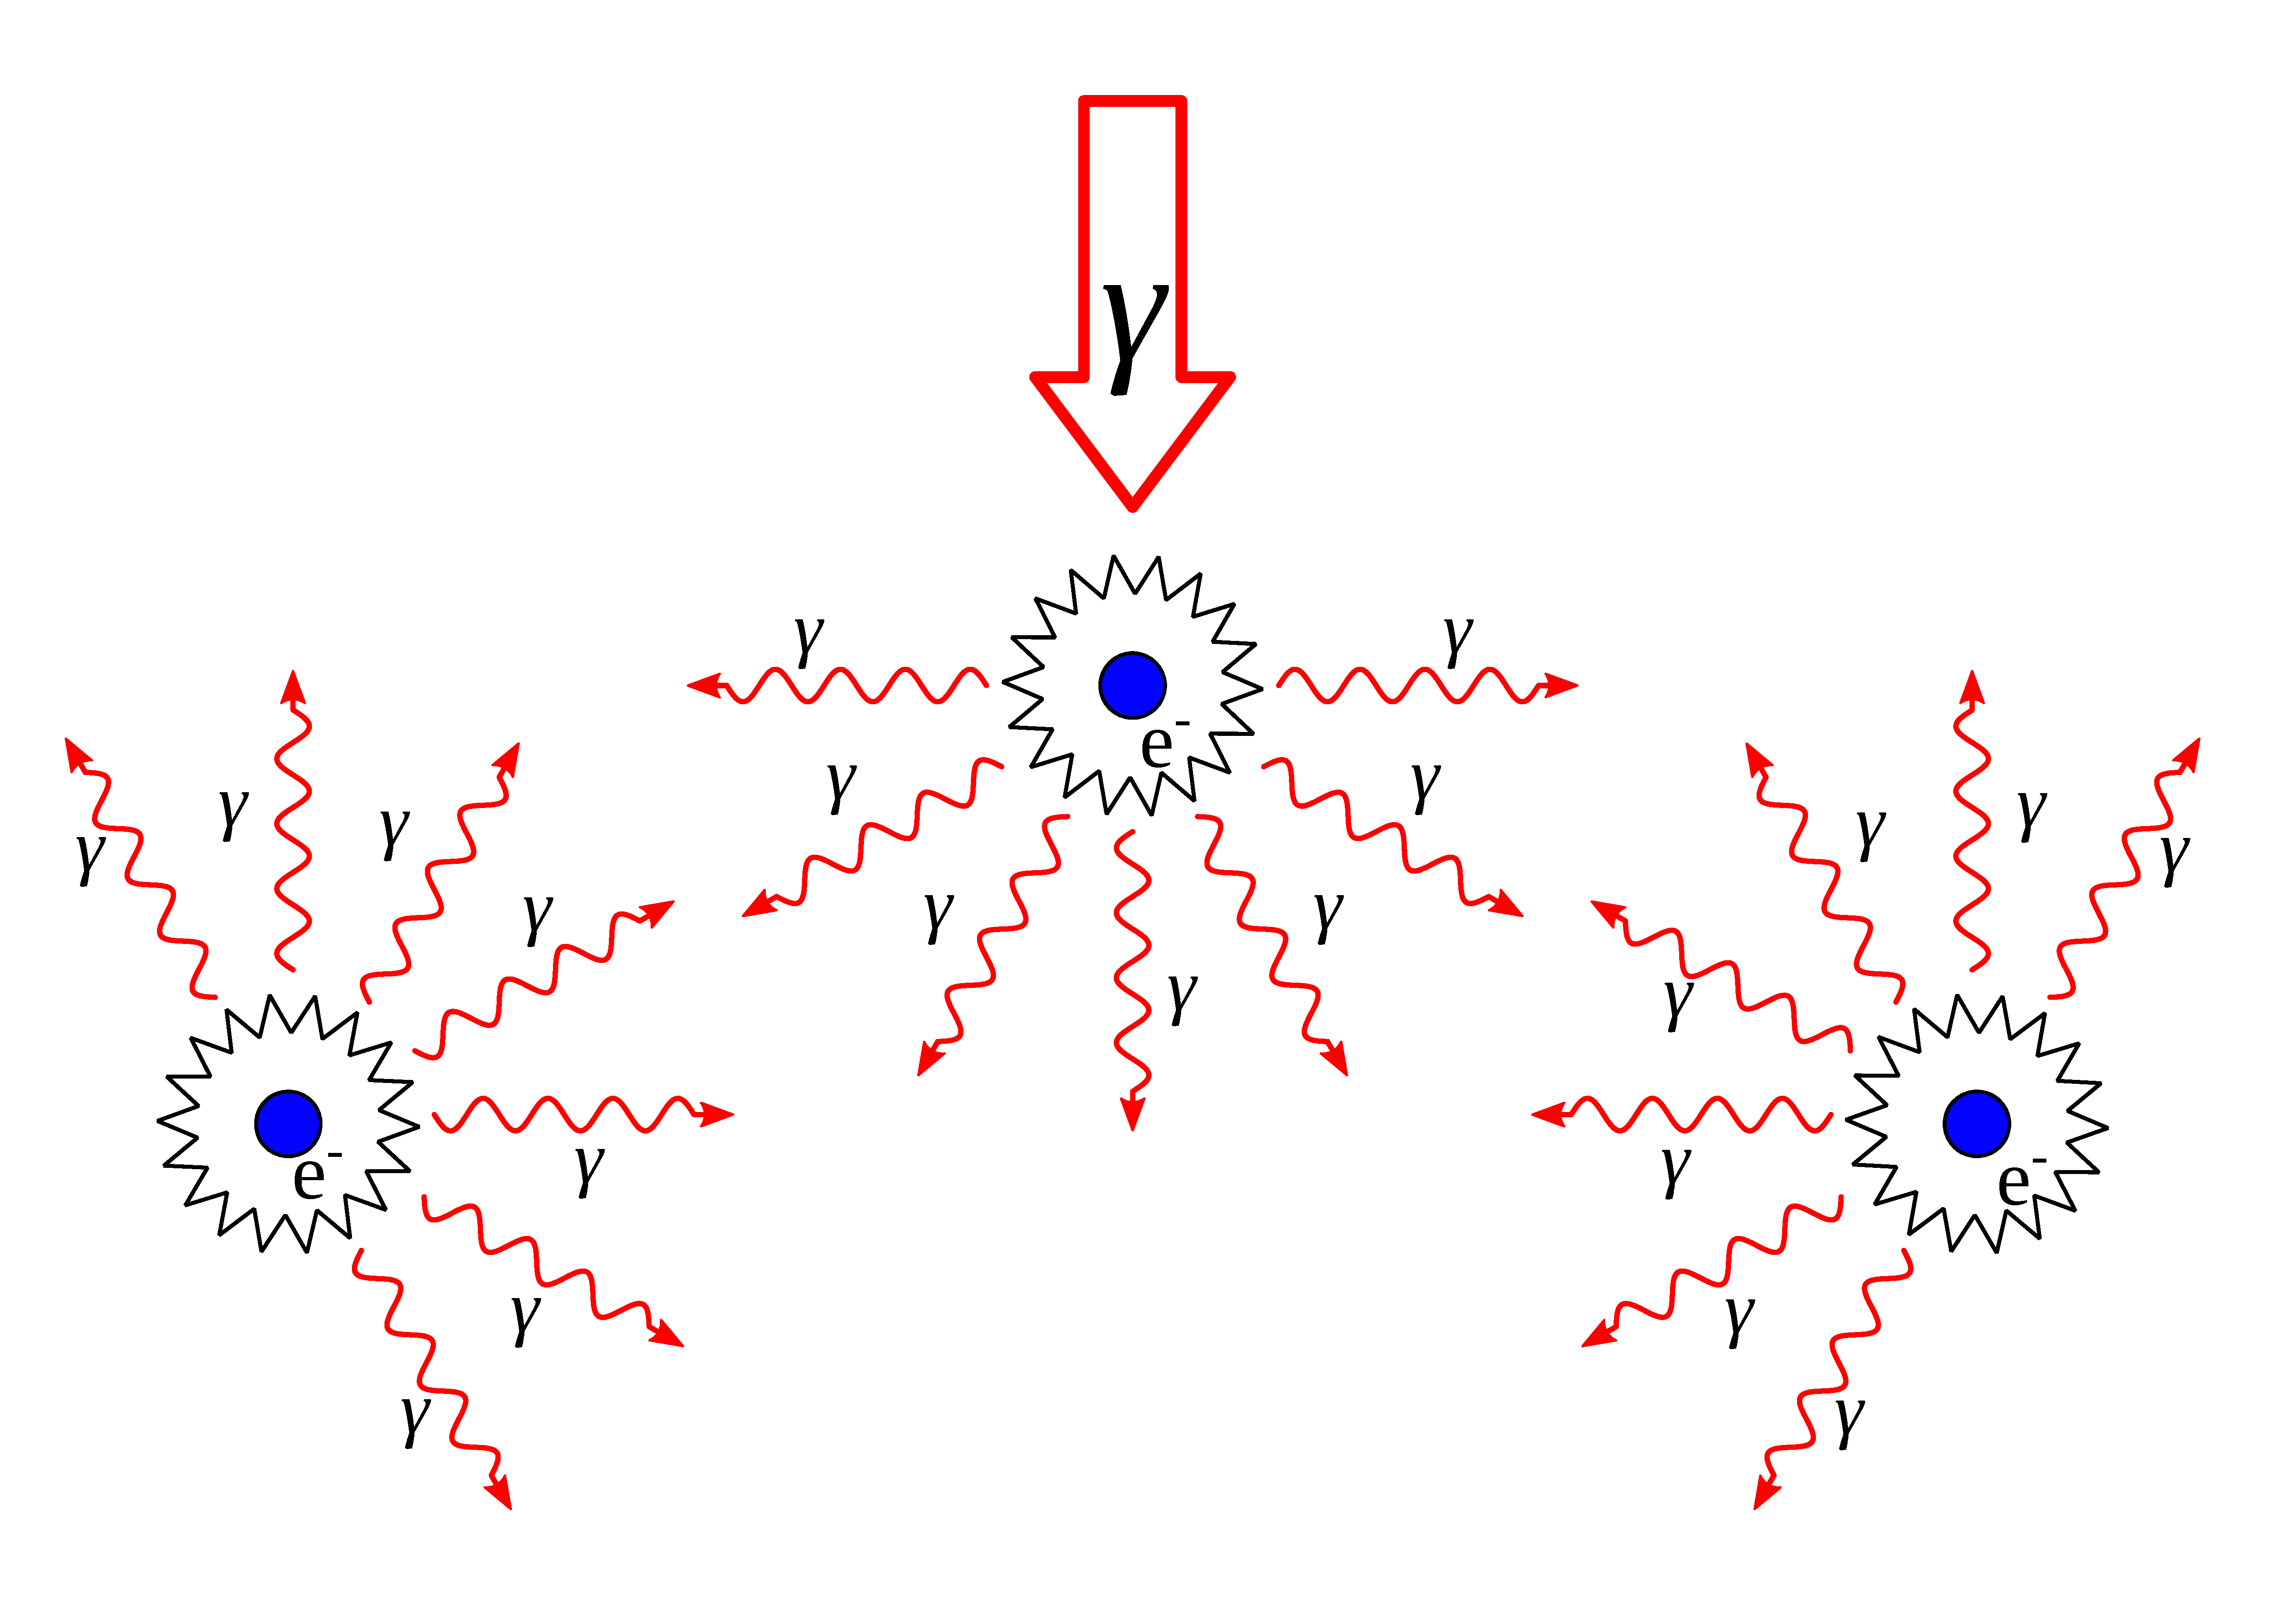
\includegraphics[scale=.15]{figures/draw.pdf}}
    \end{overpic}
    \caption{
     Processes occurring in the RL-TGE model: gamma quanta run local acceleration processes in different parts of the cloud with a multidirectional electric field.
    }
    \label{fig:rl}
\end{figure}
The crucial part of this work is additional account for escaping high energy gamma-rays in the acceleration process. Escaping photons with energy higher than 1 MeV could produce (via photo-effect or Compton-effect) new electrons with energy high enough to start separate acceleration process (Fig.~\ref{fig:rl} illustrates this process). These electrons are produced not in vicinity of first accelerator, but separated by free path of gamma ray which could be in the range from tens meters to several kilometers depending on the photon energy and atmosphere density (which depends on height). Thus these secondary accelerators could not be accounted by any local model. Additionally, the field map calculation shows that field directions in two points of a thundercloud separated by some distances are mostly uncorrelated, meaning that direction of new accelerator can be more or less random relative to the initial accelerator. If the size of a thundercloud is much larger than mean free path of gamma-ray, one can observe a chain reaction, where photons are produced in elementary accelerator cells with given local multiplication coefficient depending on local field strength and then create additional elementary accelerator cells in separate places (but some of photons could be absorbed without creating additional cell). Accounting for unproductive photons as well as loss of photons through borders of a thundercloud, one can get a global multiplicative coefficient. Obviously, in case global multiplication coefficient is larger than 1, one can observe an exponential rise in number of elementary accelerator cells and therefore total radiation level (gamma, infrared and neutron) and ionization. Also for coefficient slightly less than 1, one gets slow exponential decay of radiation background. The described model is not unlike chain reaction process in nuclear reactor, so it could be called reactor-like terrestrial gamma enhancement model (RL-TGE).

\section{Proof of concept}

For fast checking the potential of our idea, we considered a next simplified model:  
\begin{itemize}
	\item There is only one tuning parameter --- the local coefficient of gamma multiplication, describing state of the atmosphere (field strength and distribution as well as density);
	\item The number of produced of photons in a cell follows Poisson distribution, direction of momentum of a generated gamma is defined by the electric field direction;
	\item Electric field is chaotic: direction of field in cell ignition point is generated by spatial uniform distribution, but magnitude is a constant for the whole cloud;
	\item Energy of particle is not taken into account, propagation of gamma is simulated with exponential distribution with fixed mean free path;
	\item Cloud size (meaning the volume with the field) could be varied, but as a reference we take one kilometer cube, we do not track particles outside the field volume. 
\end{itemize}
This model is implemented as program\footnote{\url{https://bitbucket.org/mipt-npm/skysim/src/default/}}  on Kotlin\footnote{\url{https://kotlinlang.org/}} programming language. 

\section{Results \& Discussion}

As expected, the simulation give different result depending on the local coefficient of gamma multiplication. 
\begin{itemize}
    \item Small values of local multiplication coefficient (sub-critical mode), the reactor does not develop and number of photons decreases rather rapidly.
    \item For cell production rate of about 1.7, the avalanche could go both ways and rather develop slowly (with the characteristic time up to seconds).This regime could at least partially describe regular TGE phenomena.
    \item Multiplication higher than 1.8 generated very fast exponential rate growth (critical regime or reactor explosion). This regime gives a good explanation of TGF and could possibly be used to generate conditions for lightning discharge.
\end{itemize}

Some of the most interesting simulation results are shown in the figures. Fig.~\ref{pic-tgf-a} shows the case of an explosive growth in the number of secondary photons that are well suited to the phenomenon of TGF. Fig.~\ref{pic-ext-b}  demonstrates the case when there was a dissipation of an avalanche that had just begun to develop. Fig.~\ref{pic-tge-a}  demonstrates the case of a slower and less intensive growth. Such processes with some minor adjustments and assumptions about field dynamics could describe TGE phenomenon.

It should be noted that in general case the local multiplication coefficient is not uniform and could differ in different cloud regions. We use its averaged value. For example, if there is a local discharge and in some point of cloud the coefficient drops to zero, that average value diminish only slightly and acceleration processes in cloud won't stop.

Another important result that relates the intensity of high-energy particle production processes with cloud processes should be noted. A small change in the local coefficient of gamma multiplication is enough to go from TGE to TGF or to lightning, which leads to the two possibilities: firstly, we can describe the processes of lightning generation or the formation of TGF as a result of jumps of the local coefficient of gamma multiplication caused by fluctuations of the state of the cloud, and secondly, we can consider the cloud as a self-regulating system in which the local increase coefficient of gamma multiplication leads to activation any stopping mechanisms (for example, microdischarges that do not start global processes, but reduce the local coefficient of gamma multiplication due to the local decrease of the electric field), which allows a thunderstorm cloud to exist in sub-critical mode.

\begin{figure}[ht!]
\begin{minipage}[t]{0.45\textwidth}
		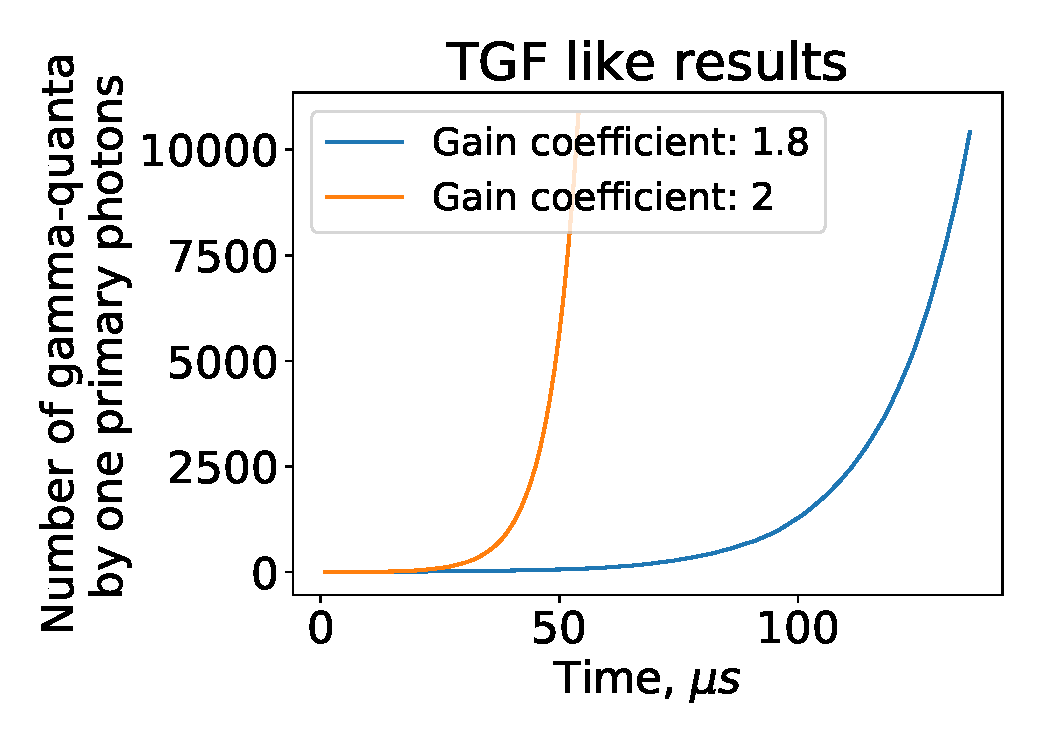
\includegraphics[width=0.95\linewidth]{figures/proofTGF.pdf}
		\caption{
		Intensive increase in the number of particles in the cloud
		}
		\label{pic-tgf-a}
\end{minipage}\hfill%
\begin{minipage}[t]{0.45\textwidth}
		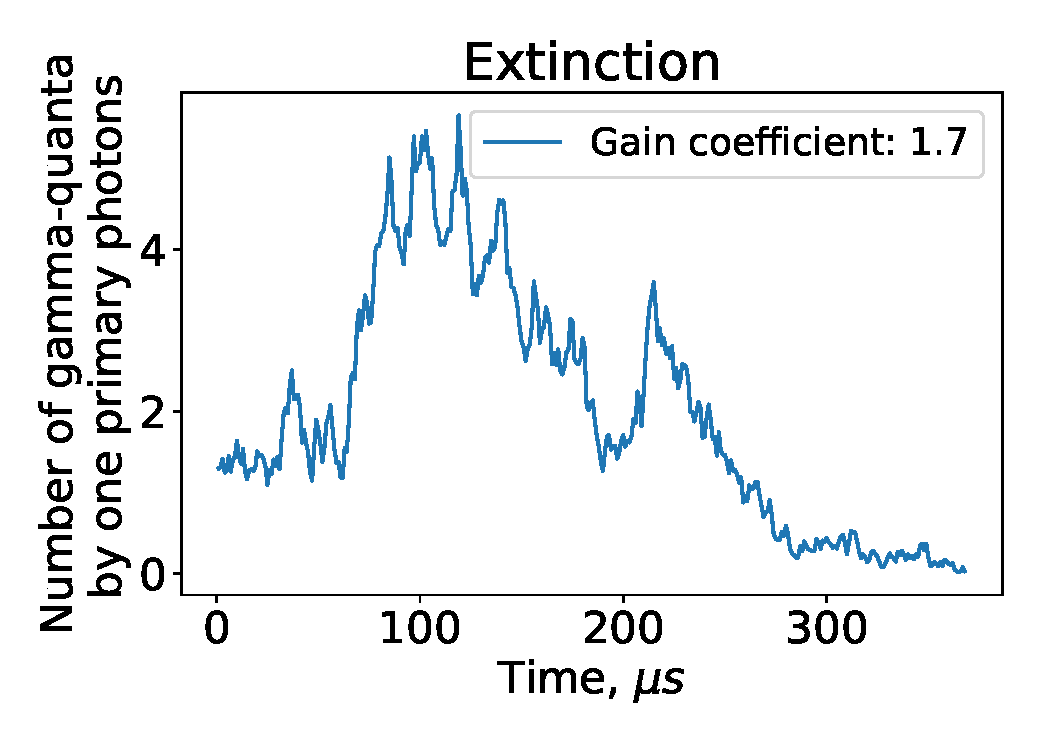
\includegraphics[width=0.95\textwidth]{figures/Extinction.pdf}
		\caption{
		An example of the attenuation of processes in the cloud
		}
		\label{pic-ext-b}
\end{minipage}
\end{figure}

\begin{figure}[ht!]
\begin{minipage}[t]{0.45\textwidth}
		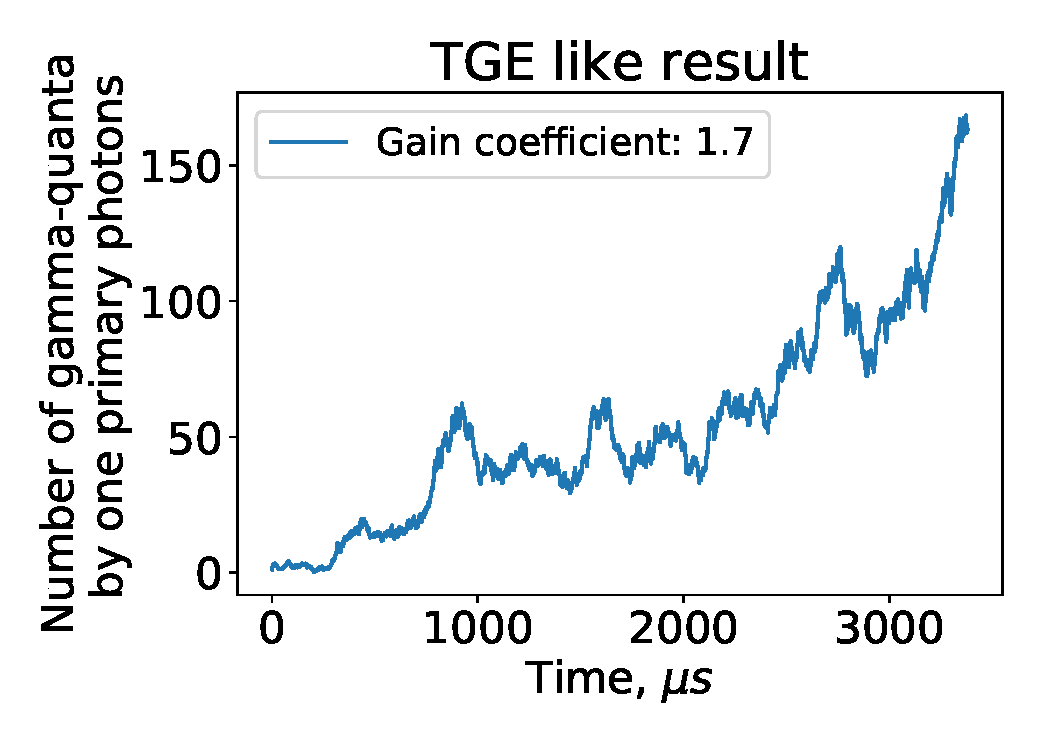
\includegraphics[width=0.95\linewidth]{figures/proofTGE.pdf}
		\caption{
		An example of a stable process in the cloud
		}
		\label{pic-tge-a}
\end{minipage}\hfill%
\begin{minipage}[t]{0.45\textwidth}
		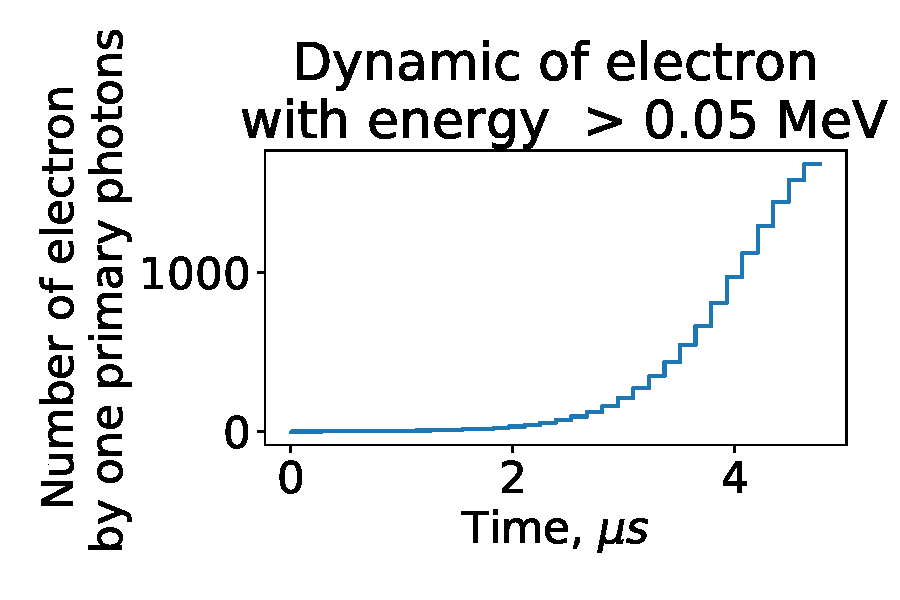
\includegraphics[width=0.95\textwidth]{figures/kotlinElectron.pdf}
		\caption{
		Intensive growth of  number of relativistic electron in prototype of improved model
		}
		\label{pic-electron-b}
\end{minipage}
\end{figure}

\section{Perspectives}

Our simple implementation of reactor like model shows potential possibility for explain the TGE phenomena, but it uses a mean value of parameter. 
Improved model clarifies rough approximations of simple model, namely:
\begin{itemize}
	\item For generating electric field map used fractal model developed by Dr. Iudin~\cite{Iudin:2018};
	\item The photons cross-section and energy-angular distribution sampling  is computed exactly, for tracking used algorithm of maximal cross-section;
	\item The spectrum of secondary particles from burned cell is simulated by GEANT4~\cite{ALLISON2016186}.
\end{itemize}

Also we improved output simulation information and parallelized calculations. By now we conduct only first simulation with improved model and we can only say, that conclusion from simple model  was confirmed. For example Fig.~\ref{pic-electron-b} shows evolution of number of relativistic electron for a small time interval.
\section{Conclusions}
\begin{itemize}
   	\item Reactor-like model is very good to describe TGF and other fast processes. For example, TGF might be turned on by thundercloud collision with the subsequent mixing of electric field lines and increase in electric field volume;
   	\item Slow processes like TGE could be described with additional assumptions about field dynamics;
   	\item The model could describe both TGE and TGF with the same mechanism depending on the state of the cloud.
\end{itemize}

Also reactor like model give next experimentally verifiable consequences:
\begin{itemize}
   	\item Contrary to Dweyer and unmodified Gurevitch models, reactor model predicts quasi-isotropic (according to field distribution) emittance of gamma-rays from a thundercloud. 	Measurement of the angular distribution of gamma-rays is required to prove or disprove the concept
   	\item At first approximation, the energy spectrum of photons produced in RL model does not depend on radiation intensity (the spectrum depends on cell field and intensity on cell number).
\end{itemize}
Moreover reactor like TGE model can be used to investigate intercloud interaction via gamma exchange.
\begin{acknowledgments}
This work is supported by the Russian Science Foundation under grant No. 17-12-01439.
\end{acknowledgments}
\nocite{*}
\bibliography{references}% Produces the bibliography via BibTeX.
\end{document}
%
% ****** End of file aipsamp.tex ******
